\section{\texttt{validationCycle}}\label{sec:example_tga}

This is the last and more complex of all \Queso{} examples. 
In this example, we numerically solve a statistical inverse problem related to a thermogravimetric experiment, where a material sample has its mass measured while loosing it through a controlled heating process. 

Given a simple mass evolution model that has a temperature profile and material properties as input parameters, and given thermogravimetirc measurements with prescribed variances, the statistical inverse problems ask for the specification of the random variables that represent the unknown material properties. We compute probability density functions with the Bayesian approach and
compute sets of realizations through the Metropolis-Hastings algorithm with delayed rejection.
% DRAM Markov chain algorithm.
%Once the random variables are computed, they become input parameters on statistical forward problems,
%which ask for the statistical prediction of the sample mass evolution under a specified temperature profile.
%We solve the statistical forward problems with the Monte Carlo algorithm.

We qualitatively analyse the sensitivity of the solutions
with respect to problem characteristics,
namely ``amount'' of data and ``quality'' of data, and also
with respect to algorithm options,
namely chain initial position, number of delayed rejections
%, covariance matrix adaptivity
and chain size.




\subsection{Thermogravimetric Experiments and a Simple Model}

Suppose a given material sample of initial mass $m_0$ and at initial temperature $T_0$ is heated with constant heating rate $\beta$ (K/min). Heating is maintained until the sample fully ablates (decomposes). The sample mass $m(T)$ is measured at temperatures $T>T_0$.
Let $w(T)~=~m(T)/m_0$ denote the mass fraction.

% 
% A material sample with initial mass $m_0$ and at initial temperature $T_0$ is heated
% with constant heating rate $\beta$ (K/min) until it fully decomposes.
% Let $w(T)=m(T)/m_0$ denote the mass fraction.
\begin{figure}[!h]
\centering
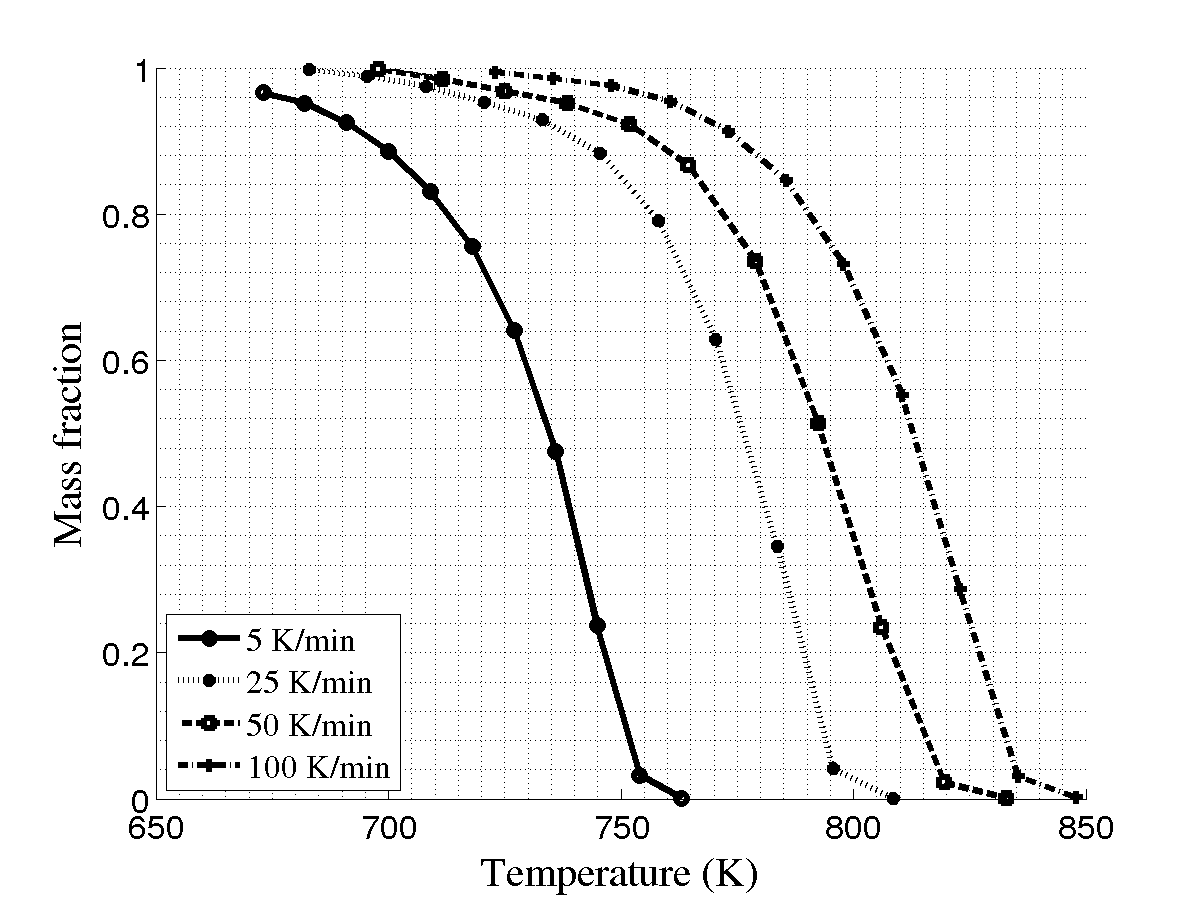
\includegraphics[scale=0.4]{figs/tga_experiment_data.png}
\vspace*{-8pt}
\caption{Mass fraction decay over temperature given different heating rates. Data from J. A. Conesa, R. F. Marcilla and J. A. Caballero, ``Thermogravimetric studies on the thermal decomposition of polyethylenes'', {\it J. Anal. Appl. Pyrolysis}, 36(1):1-15, 1996}
\label{fig:tga-exp-data}
\end{figure}


It is convenient to transform the kinetic equation to a \emph{per unit temperature} form by dividing through by
$\beta$. Thus, a simple approach to the simulation of a thermogravimetric phenomenon consists on modelling the sample as a
homogeneous material of scalar properties $A>0$ and $E>0$ whose relative mass $w$ obeys the following initial value ordinal differential equation problem:
\begin{equation}\label{eq:tga-model}
\left\{
\begin{array}{rcll}
{\displaystyle \frac{dw}{dt} } & = & -\dfrac{A w}{\beta} \exp\left(-\frac{E}{RT}\right), & t \geqslant 0,\\
& & \\
w(0) & = & 1, &
\end{array}
\right.
\end{equation}
where the kinetic parameters $A$ and $E$ are referred to, respectively, as pre-exponential factor (min$^{-1}$) and activation energy (J/mol).


In this combined SIP--SFP, we  calibrate both model parameters $A$ and $E$ given the mathematical model in Equation \eqref{eq:tga-model} and experimental data (Section \ref{sec:tga-data}). Then the inferred values for $A$ and $E$ are then used for uncertainty propagation on the remaining mass fraction at time $t=3.9$ s when $\beta=250$ K/min, i.e., our quantity of interest is $w(t=3.9)$. 

\subsection{Statistical Inverse Problem}\label{sec:tga-sip}

%
Let $\mathbf{m}=(A,E)$ be the vector of model parameters and $M=\mathbb{R}_{+}^{2}$ be the space of model parameters.
Let
$V_T$ denote the space of functions $f:\mathbb{R}_{+}\rightarrow\mathbb{R}_{+}$ that are weakly differentiable.
$V_T$ will be the space of temperature profiles.
Finally, let
$V_w$ denote the space of functions $f:\mathbb{R}_{+}\rightarrow[0,1]$ that are weakly differentiable.
$V_w$ will be the space of relative mass evolutions.
We will denote by
\begin{equation*}
w(\mathbf{m},T)\in V_w
\end{equation*}
the solution of Equation \eqref{eq:tga-model} for given $\mathbf{m}\in M$ and $T\in V_T$.


% 
% This model can be easily generalized to a sample composed of $N_{\text{mat}}\geqslant 1$ materials. We refer to \cite{eep_ices_rep1} for details.

\subsubsection{Misfit Functions $\mathcal{F}(\mathbf{m})$}

Let
$V_S$ denote the space of all functions $f:\mathbb{R}_{+}\rightarrow\mathbb{R}_{+}$ that are square-Lebesgue-integrable
over any finite interval.
$V_S$ will be the space of misfit weight functions.
Let
$V_{\sigma}$ denote the space of all functions $f:\mathbb{R}_{+}\rightarrow\mathbb{R}_+^{*}$ such that $1/f$ is square-Lebesgue-integrable
over any finite interval.
$V_{\sigma}$ will be the space of variance functions.

Given a reference relative mass evolution function $\text{$d$}\in V_w$,
a temperature profile $T\in V_T$,
and some $t_{_{\text{F}}}>0$,
let $\mathcal{F}:M\rightarrow\mathbb{R}$ be the functional defined by
\begin{equation*}
\mathcal{F}(\mathbf{m}) = \int_{0}^{t_{_{\text{F}}}}~\left\{[w(\mathbf{m},T)](t)-\text{$d$}(t)\right\}^2\cdot S(t)~dt,
\end{equation*}
or simply
\begin{equation}\label{eq-F}
\mathcal{F}(\mathbf{m}) = \int_{0}^{t_{_{\text{F}}}}~(w-d)^2\cdot S~dt.
\end{equation}


The functional \eqref{eq-F} is general enough for our studies, since it can properly describe
not only the case where one has continuous measurements $\text{$d$}$,
but also the case of a finite set of $N_{\text{meas}}$ discrete measurements $0\leqslant d_j\leqslant 1$,
$1\leqslant i\leqslant N_{\text{meas}}$ at instants $0\leqslant t_1 < t_2 < \ldots < t_{N_{\text{meas}}}$.

In the case of continuous measurements, for instance, one can set
\begin{equation*}
\mathcal{F}_1(\mathbf{m}) = \int_{0}^{t_{_{\text{F}}}}~\left\{[w(\mathbf{m},T)](t)-\text{$d$}(t)\right\}^2\cdot\frac{1}{\sigma^2(t)}~dt,
\end{equation*}
for some given variance function $\sigma^2\in V_S$ satisfying $\sigma(t)>0$ for all $t\geqslant 0$.

On the other hand, when measurements are discrete and a corresponding finite set of variances $\sigma_j^2>0,~j=1,2,\ldots,N_{\text{meas}}$ is given, one can set
\begin{equation*}
\mathcal{F}_2(\mathbf{m}) = \int_0^{t_{_F}}~\{[w(\mathbf{m},T)](t)-\hat{d}(t)\}^2\cdot\left[\sum_{j=1}^{N_{\text{meas}}}\frac{\delta(t-t_j)}{{\hat{\sigma}}^2(t)}\right]~dt,
\end{equation*}
where
$\hat{d}\in V_w$ and $\hat{\sigma}\in V_{\sigma}$ are any functions satisfying
$\hat{d}(t_j)=d_j$ and $\hat{\sigma}(t_j)=\sigma_j$, $j=1,2,\ldots,N_{\text{meas}}$,
in which case the functional simply becomes
\begin{equation*}
\mathcal{F}_2(\mathbf{m}) = \sum_{j=1}^{N_{\text{meas}}}~\frac{\{[w(\mathbf{m},T)](t_j)-d_j\}^2}{\sigma_j^2},
\end{equation*}
assuming, without loss of generality, that $t_{_F}\geqslant t_{N_{\text{meas}}}$.

\subsubsection{Bayesian Approach: Prior RV, Likelihood and Posterior RV}


In \underline{deterministic} inverse problems treat the unknown parameters as scalars or vectors and the goal is
the calculation of their best values according to a given criteria, usually least squares, e.g. solving the unconstrained optimization problem
\begin{equation}\label{eq-unconstrained-min}
\underset{\mathbf{m}\in M}{\text{min}}~\mathcal{F}(\mathbf{m}).
\end{equation}

In \underline{statistical} inverse problems, the unknown parameters are treadted as random variables (rvs) and the goal is the specification of their probability density functions (pdfs)~\cite{KaSo05}.




Applying the Bayesian approach
\begin{equation*}
\pi_{\text{posterior}}(\mathbf{m})\propto \pi_{\text{prior}}(\mathbf{m})\cdot\pi_{\text{likelihood}}(\mathbf{m})
\end{equation*}
we have that for the TGA SIP, the prior distribution and the likelihood are, respectively:
\begin{equation*}
\pi_{\text{prior}}(\mathbf{m}) \propto e^{-\frac{1}{2}V(\mathbf{m})}\quad\text{and}\quad
%
\pi_{\text{likelihood}}(\mathbf{m}) \propto e^{-\frac{1}{2}\mathcal{F}(\mathbf{m})}.
\end{equation*}


Thus, we chose parameters $(A,E)$ to have joint uniform prior pdf over the open square domain, i.e.:
$$\pi_{\text{prior}}=\mathcal{U}((1.0\times 10^{10},5.0\times 10^{11})\times (4.0\times 10^{5},6.0\times 10^{5})).$$



\subsubsection{Data from experiments}\label{sec:tga-data}

Table \ref{table:data-tga} presents the data collected in the TGA experiment. 

\begin{table}[htb]
\begin{center}
\begin{tabular}{cllc}
\toprule
Observation   & Temperature     & Relative mass             & Variance \\
index ``$i$'' & $T_i$ (K)       & $m^*_{\text{obs},i}$ (\%) & $V_i$    \\
\midrule
\midrule
 1            & $\quad$ 673.034 & $\quad$ 96.5855    & 0.1      \\
 2            & $\quad$ 682.003 & $\quad$ 95.1549    & 0.1      \\
 3            & $\quad$ 690.985 & $\quad$ 92.5048    & 0.1      \\
 4            & $\quad$ 699.979 & $\quad$ 88.6353    & 0.1      \\
 5            & $\quad$ 708.989 & $\quad$ 83.0585    & 0.1      \\
 6            & $\quad$ 718.02  & $\quad$ 75.5306    & 0.1      \\
 7            & $\quad$ 727.089 & $\quad$ 64.1003    & 0.1      \\
 8            & $\quad$ 735.96  & $\quad$ 47.5474    & 0.1      \\
 9            & $\quad$ 744.904 & $\quad$ 23.6777    & 0.1      \\
 10           & $\quad$ 754.062 & $\quad$ 03.2234    & 0.1      \\
 11           & $\quad$ 763.049 & $\quad$ 00.0855448 & 0.1      \\
\bottomrule
\end{tabular}
\vspace{-.2cm}
\caption{Experimental data.}\label{table:data-tga}
\end{center}
\end{table}

\subsection{Statistical Forward Problem}\label{sec:tga-sfp}

In spacecraft design, ablation is used to both cool and protect mechanical parts and/or payloads that would otherwise be damaged by extremely high temperatures. Two principal applications are heat shields for spacecraft entering a planetary atmosphere from space and cooling of rocket engine nozzles~\cite{wiki:ablation}. 

Suppose that a object about to re-enter the Earth atmosphere has a thermal protection layer (shield) of composition of the same sample material described in Section \ref{sec:tga-sip}. Also, as the object re-enters the atmosphere, its shield loses mass accorging to Equation \eqref{eq:tga-model}.  The initial sample temperature is $T_0=0.1$ K and it is then heated with constant rate $\beta=5$ K/m.
% We are interested in answering a few questions:
% \begin{enumerate}
%  \item At scenario $\beta=250$ K/min, what is the remaining mass fraction at time $t=3.9$ s, i.e. $$w(t=3.9s)?$$
%  \item Supposing that a failure occurs when the remaining mass fraction is smaller than 20\%, what is the probability of failure at time $t=3.9$ s, i.e. $$P(w(t=3.9s)<0.2)?$$
%  \item  Supposing that the probability of failure is $\leq 5\%$, what is the margin in the prediction of the probability of failure?
% \end{enumerate}

We are interested in answeing the following question: at scenario $\beta=250$ K/min, what is the remaining mass fraction at time $t=3.9$ s? In other words, the quantity of interest is $w(t=3.9s)$.



% \todo{Suppose also that, under such conditions, our quantity of interest (QoI) is the time necessary to the sample to ablate 75\% of its mass, denoted by $t_\text{0.25}$ (s). In other words, we are interested in estimate how long it takes for $w=0.25$, or}
% \begin{equation}
%  \text{Find } t_\text{0.25} \text{ such as } w(t_\text{0.25} )=0.25
% \end{equation}

\subsubsection{The Input RV, QoI Function and Output RV}


The input random variables for this SFP are the inferred parameters $A$ and $E$ which are the solution (posterior PDF) of the inverse problem described in Section \ref{sec:tga-sip}. The output random variable for this example is the remaining mass fraction at 3.9 s, i.e. $w(t=3.9)$. Note that, since there is uncertainty in the parameters $A$ and $E$ (both given as PDFs), one can expect that this uncertainty will be propagated to $w(t=3.9)$, which will also be given as a PDF. Finally, the QoI function for $w$ is the solution of the Equation \eqref{eq:tga-model} evaluated when $t=3.9$ s, which is calculated using numerical integration with adjustable and acceptable time-stepping using GSL function \verb+gsl_odeiv_evolve_apply+\footnote{\url{http://www.gnu.org/software/gsl/manual/html_node/Evolution.html\#index-gsl_005fodeiv2_005fevolve_005fapply}}. 

\subsection{Running the Example}\label{sec:tga-run}

To run the executable provided (available after QUESO installation), and generate figures for the chains, PDFs, CDFs, etc., enter the following commands:
\begin{lstlisting}[label={},caption={}]
$ cd $HOME/LIBRARIES/QUESO-0.47.1/examples/validationCycle
$ rm outputData/*
$ ./exTgaValidationCycle_gsl tagCycle.inp    
$ matlab
   $ tga_cycle_plot.m     # inside matlab
   $ exit                 # inside matlab
$ ls -l outputData/*.png
  cal_parameter1_prior.png                cal_parameter2_prior.png                
  cal_val_parameter1_PDF.png              cal_val_parameter2_PDF.png              
  cal_val_parameter1_CDF.png              cal_val_parameter2_CDF.png              
  cal_val_parameter1_autocorr.png         cal_val_parameter2_autocorr.png
  cal_val_QoI_CDF.png                     cal_val_QoI_PDF.png
  cal_val_QoI_autocorrelation.png            
\end{lstlisting}
% cal_val_QoI_CDF_model_confidence_full.png
% cal_val_QoI_CDF_model_confidence_zoom.png


As a result, the user should have created several of PNG figures containing marginal posterior PDF, chain positions of the parameters and the QoI, histogram, cumulative density distribution and autocorrelation. The name of the figure files have been chosen to be informative, as shown in the Listing above.



\subsection{TGA Example Code}\label{sec:code-tga}



The program example given in this paper is compatible with version 0.47.1 of QUESO.
The source code for the example is composed of 5 files:
 \texttt{exTgaValidationCycle\_gsl.C} (Listing \ref{code:tga-main-c}),
 \texttt{exTgaValidationCycle\_appl.h} (Listing \ref{code:tga-appl-h}), 
 \texttt{exTgaValidationCycle\_likelihood.h}  (Listing \ref{code:tga-like-h}) and 
\texttt{exTgaValidationCycle\_qoi.C} (Listing \ref{code:tga-qoi-h}).



\lstinputlisting[caption=File \texttt{exTgaValidationCycle\_gsl.C}., label={code:tga-main-c}, linerange={30-1000}]{../../examples/validationCycle/src/exTgaValidationCycle_gsl.C}

\lstinputlisting[caption=File \texttt{exTgaValidationCycle\_appl.h}., label={code:tga-appl-h}, linerange={33-1000}]{../../examples/validationCycle/src/exTgaValidationCycle_appl.h}

\lstinputlisting[caption=File \texttt{exTgaValidationCycle\_likelihood.h.}, label={code:tga-like-h}, linerange={33-1000}]{../../examples/validationCycle/src/exTgaValidationCycle_likelihood.h}

\lstinputlisting[caption=File \texttt{exTgaValidationCycle\_qoi.h}., label={code:tga-qoi-h}, linerange={33-1000}]{../../examples/validationCycle/src/exTgaValidationCycle_qoi.h}




\subsection{Input File}\label{sec:tga-input-file}

The input file used with this TGA SIP--SFP QUESO provides QUESO with options for its enviroments, and for both  MCMC and Monte-Carlo alogothims. It is displayed in Listing~\ref{code:tga-input-file}.


\lstinputlisting[caption={File name \texttt{tgaCycle.inp} with options for QUESO library used in application code (Listings \ref{code:tga-main-c}-\ref{code:tga-like-h}})., 
label={code:tga-input-file},]{../../examples/validationCycle/tests/test_2012_11_15/tgaCycle.inp}



\subsection{Data Post-Processing and Visualization}\label{sec:tga-results}


According to the specifications of the input file in Listing~\ref{code:tga-input-file}, both a folder named \verb+outputData+ and a the following files should be generated:
\begin{verbatim}
file_cal_ip_raw.m        file_val_ip_raw.m        
file_cal_ip_raw_sub0.m   file_val_ip_raw_sub0.m
file_cal_fp_qoi2.m       file_val_fp_qoi2.m      
file_cal_fp_qoi2_sub0.m  file_val_fp_qoi2_sub0.m     
tgaCalOutput_sub0.m      tgaValOutput_sub0.m
display_sub0.txt    
\end{verbatim}


The sequence of Matlab commads is identical to the ones presented in Sections \ref{sec:sip-results}, \ref{sec:sfp-results} and \ref{sec:gravity-results}; therefore, are ommitted here. The reader is invited to explore the Matlab file \texttt{tga\_cycle\_plot.m}  
%\texttt{validationCycle/tests/test\_2012\_11\_15/tga\_cycle\_plot.m} 
for details of how the figures have been generated.

\subsubsection{KDE Plots of Parameters}
Matlab function \verb+ksdensity+ (Kernel smoothing density estimate) together with the option `\verb+pdf+' may be used to estimate the KDE of the paremeters, as illustrated in Figure \ref{fig:tga_ip_pdf}.
% \begin{figure}[htb]
% \centering 
% \subfigure{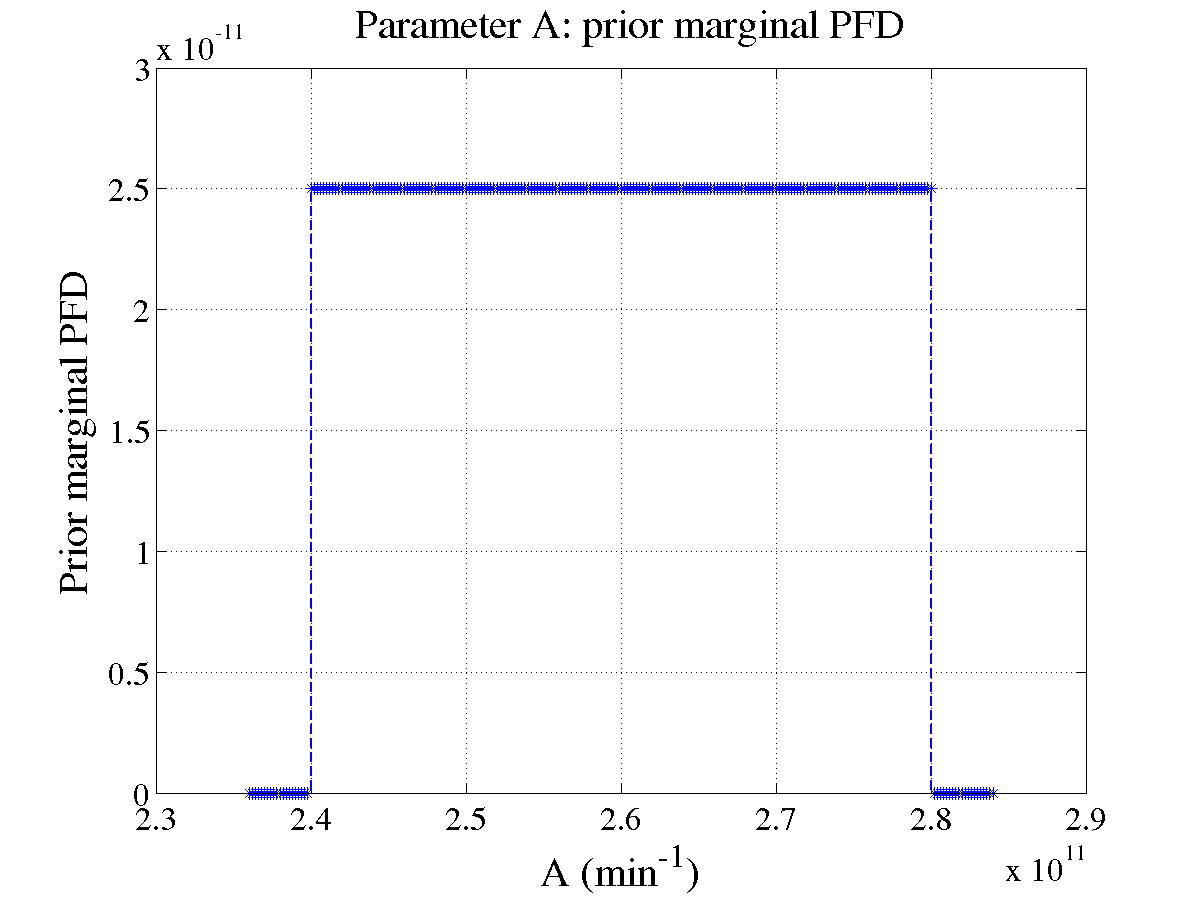
\includegraphics[scale=0.40]{figs/cal_parameter1_prior.png}}
% \subfigure{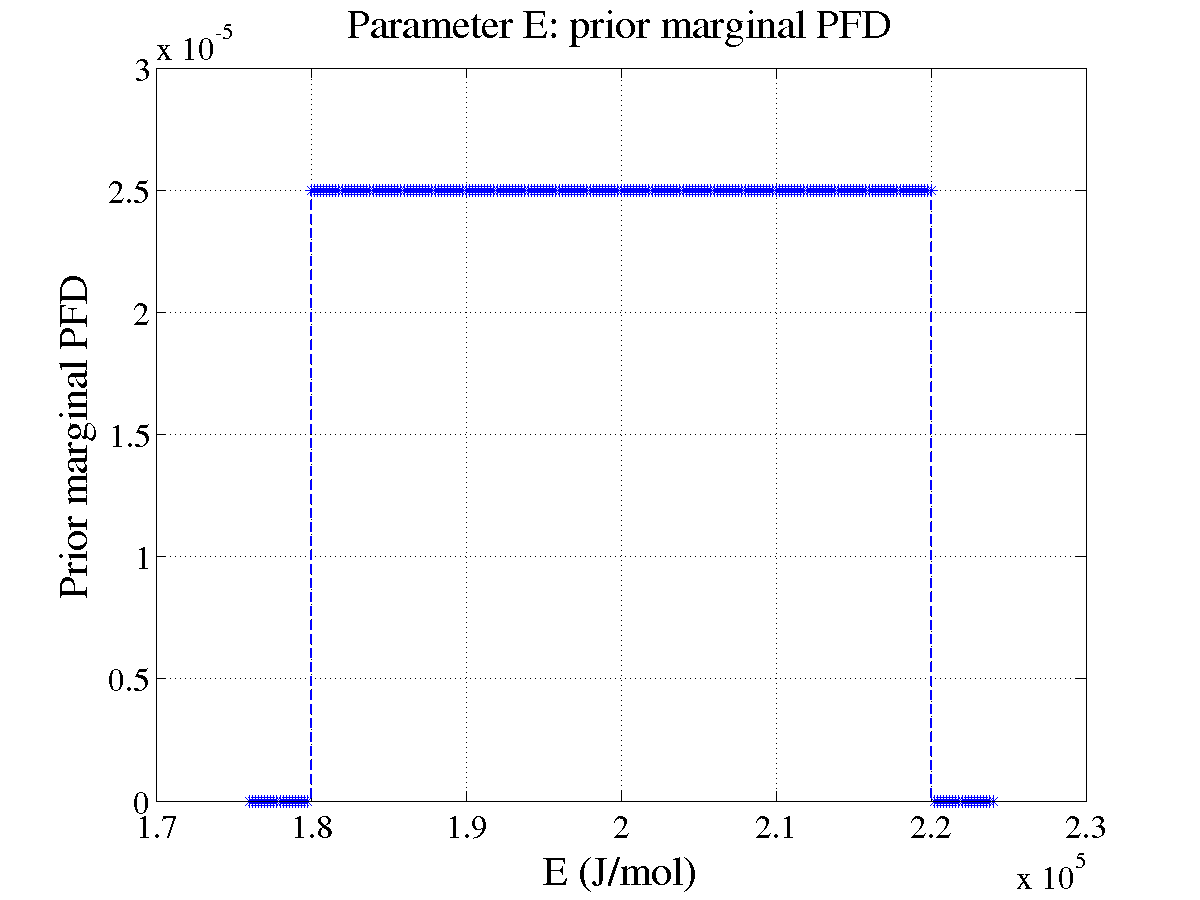
\includegraphics[scale=0.40]{figs/cal_parameter2_prior.png}}
% \vspace*{-10pt}
% \caption{Prior distributions of parameters $A$ and $E$.}
% \end{figure}
%
\begin{figure}[htpb]
\centering 
\subfigure{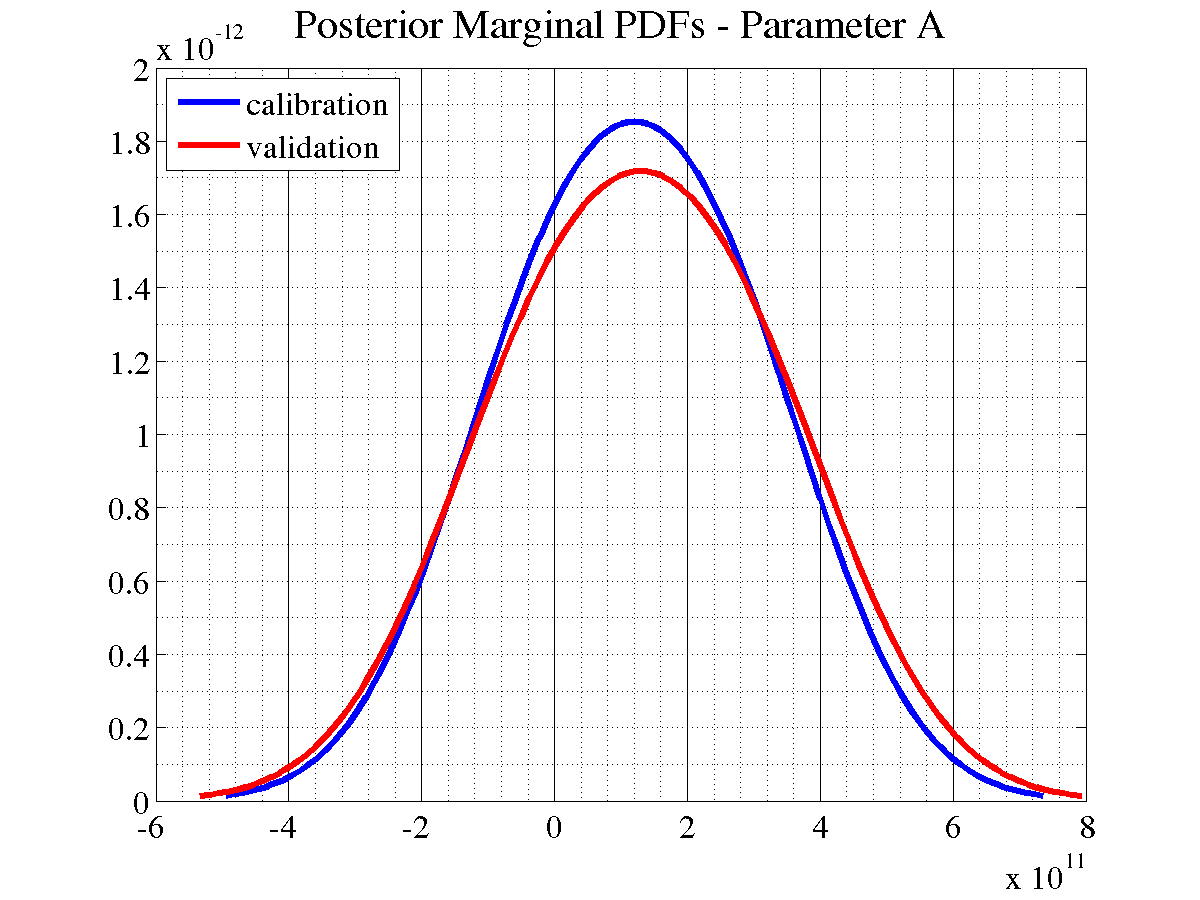
\includegraphics[scale=0.35]{figs/cal_val_parameter1_PDF.png}}
\subfigure{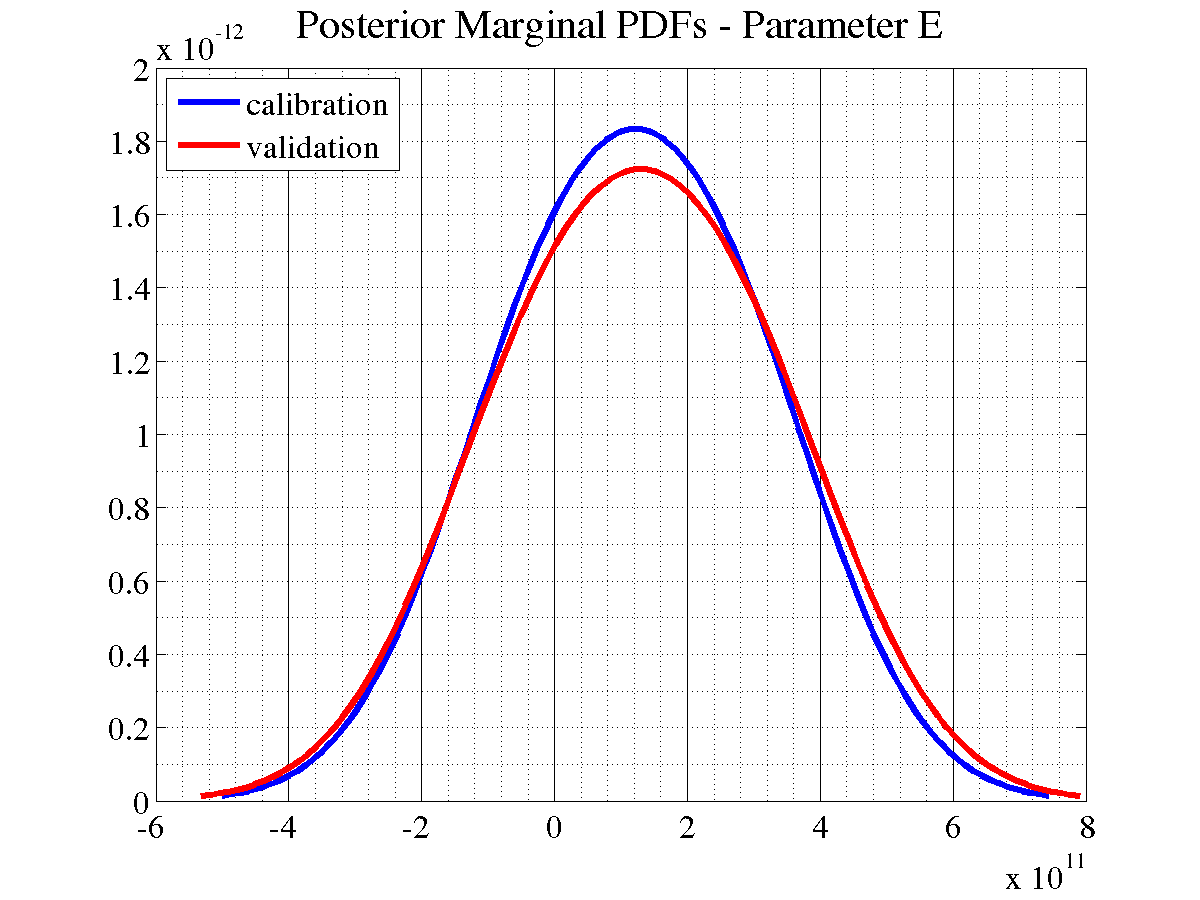
\includegraphics[scale=0.35]{figs/cal_val_parameter2_PDF.png}}
\vspace*{-10pt}
\caption{Posterior distributions of parameters $A$ and $E$.}
\label{fig:tga_ip_pdf}
\end{figure}



\subsubsection{CDF Plots of Parameters}

Matlab function \verb+ksdensity+ with \verb+'cdf'+ option may also be used for plotting the Cumulative Distribution Function of each one of the parameters, as illustrated in Figure \ref{fig:tga_ip_cdf}.
%
\begin{figure}[htpb]
\centering 
\subfigure{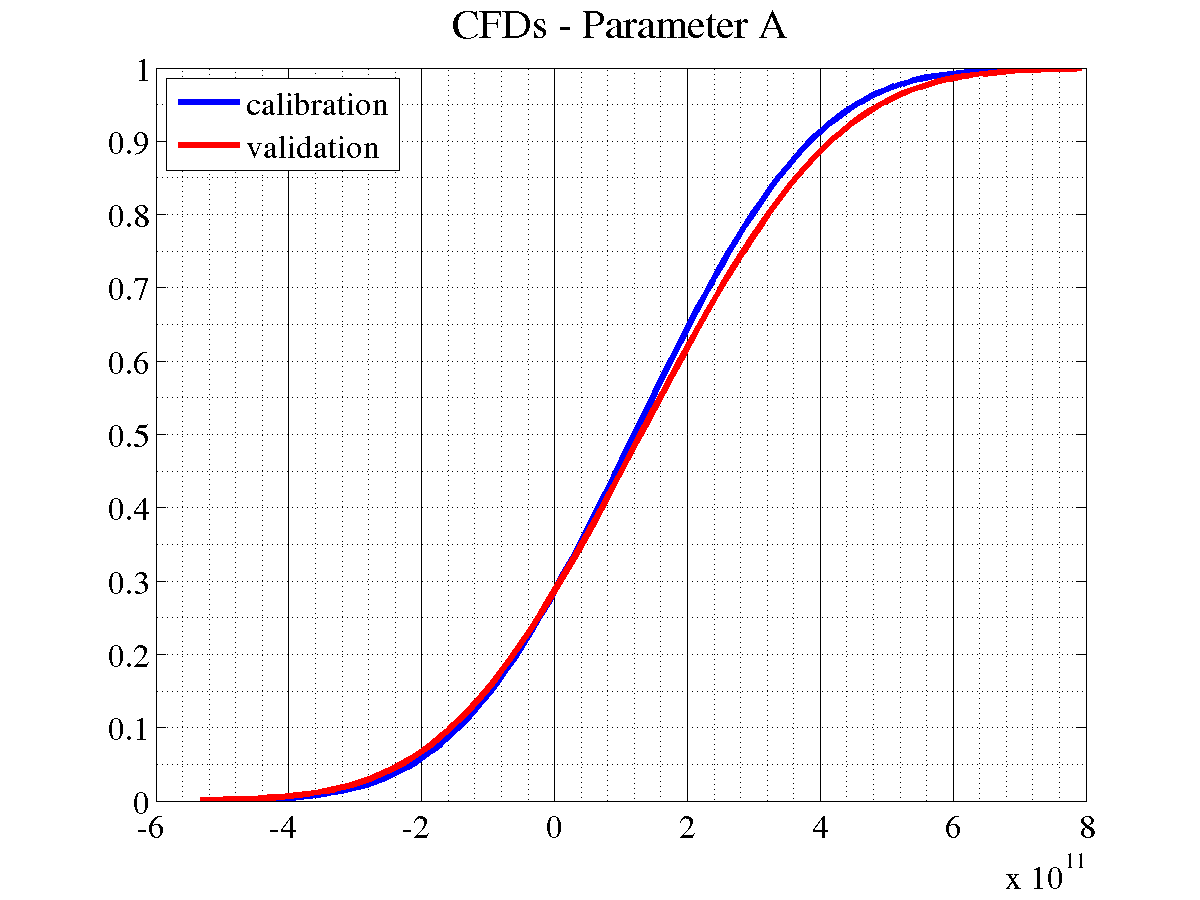
\includegraphics[scale=0.35]{figs/cal_val_parameter1_CDF.png}}
\subfigure{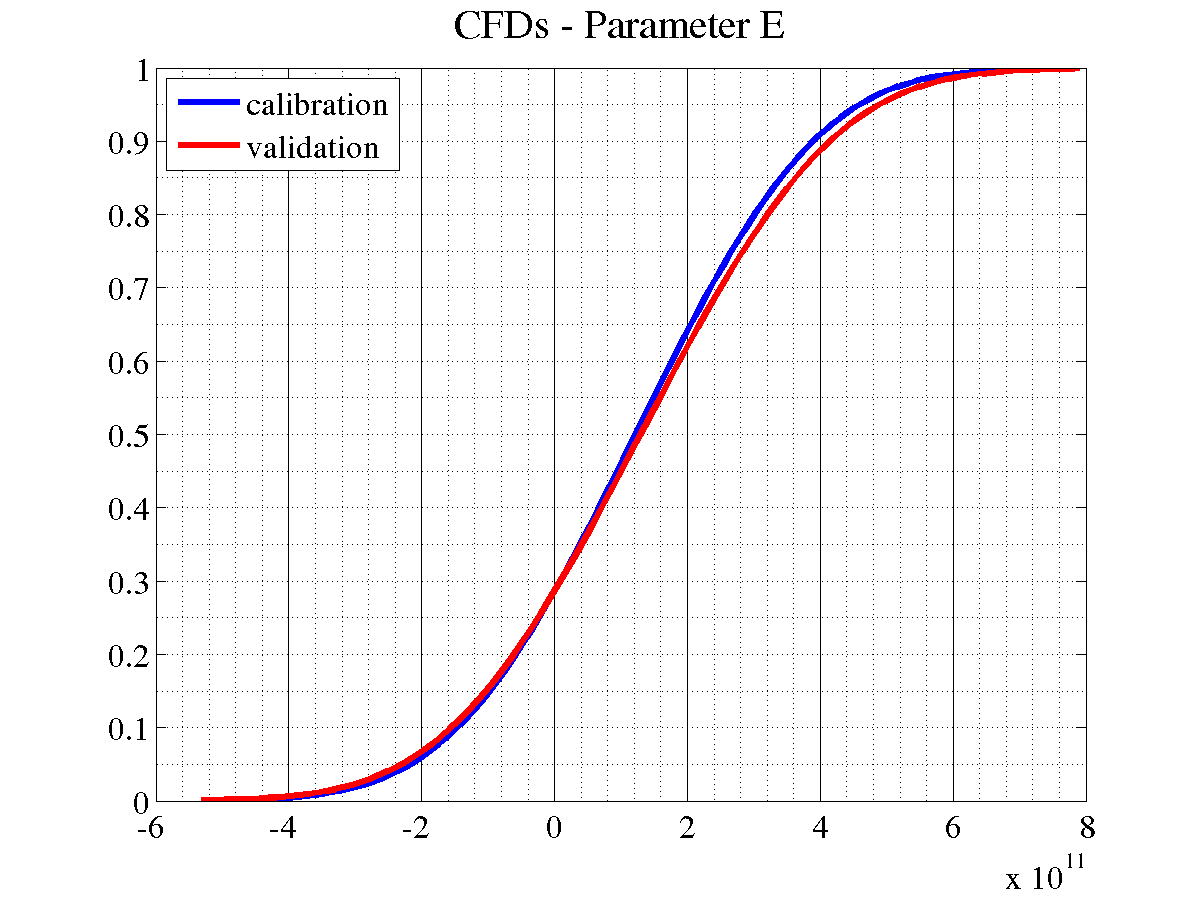
\includegraphics[scale=0.35]{figs/cal_val_parameter2_CDF.png}}
\vspace*{-10pt}
\caption{Cumulative density functions of parameters $A$ and $E$.}
\label{fig:tga_ip_cdf}
\end{figure}



\subsubsection{Autocorrelation Plots of Parameters}

Figure \ref{fig:tga_ip_autocorrelation_param} presents the autocorrelation of the parameters $A$ and $E$ in both cases: calibration and validation stages.

\begin{figure}[htpb]
\centering 
\subfigure{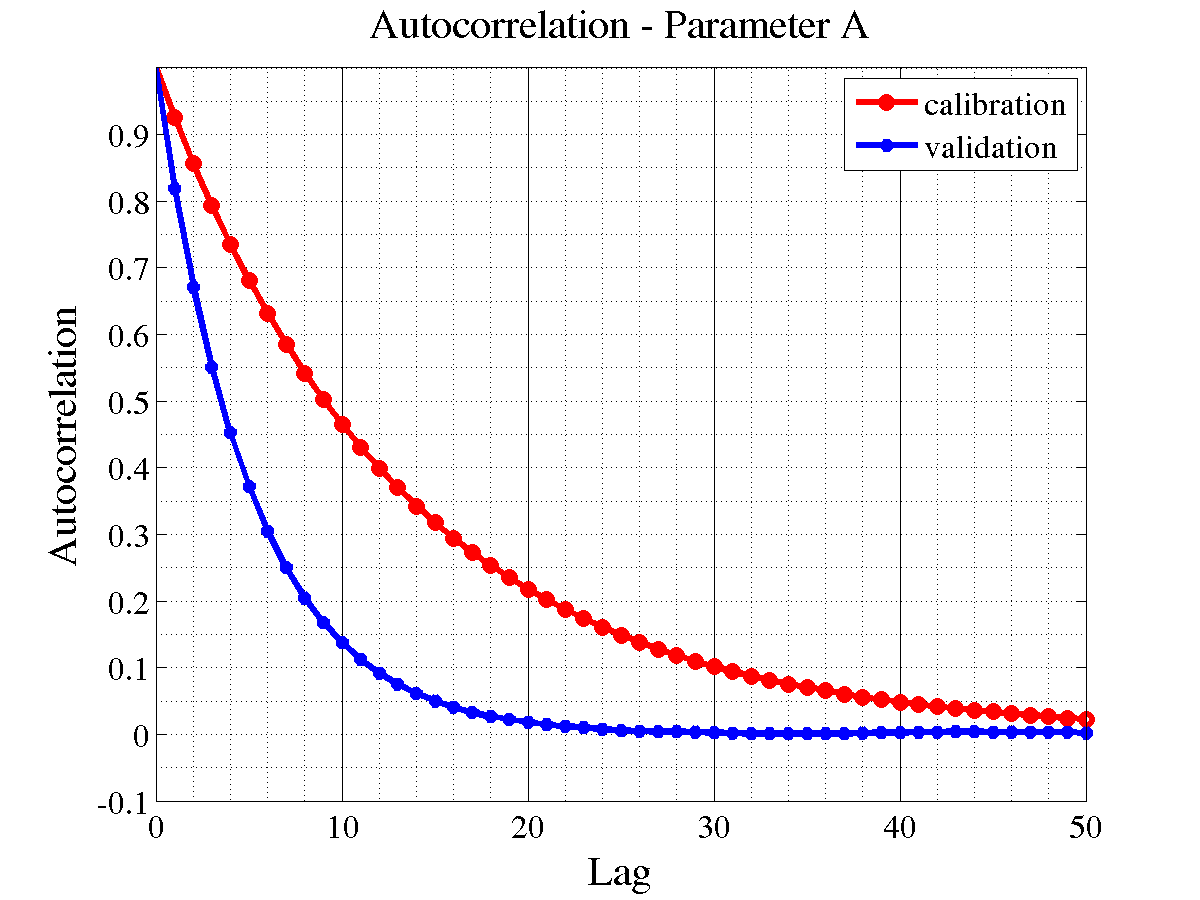
\includegraphics[scale=0.35]{figs/cal_val_parameter1_autocorrelation.png}}
\subfigure{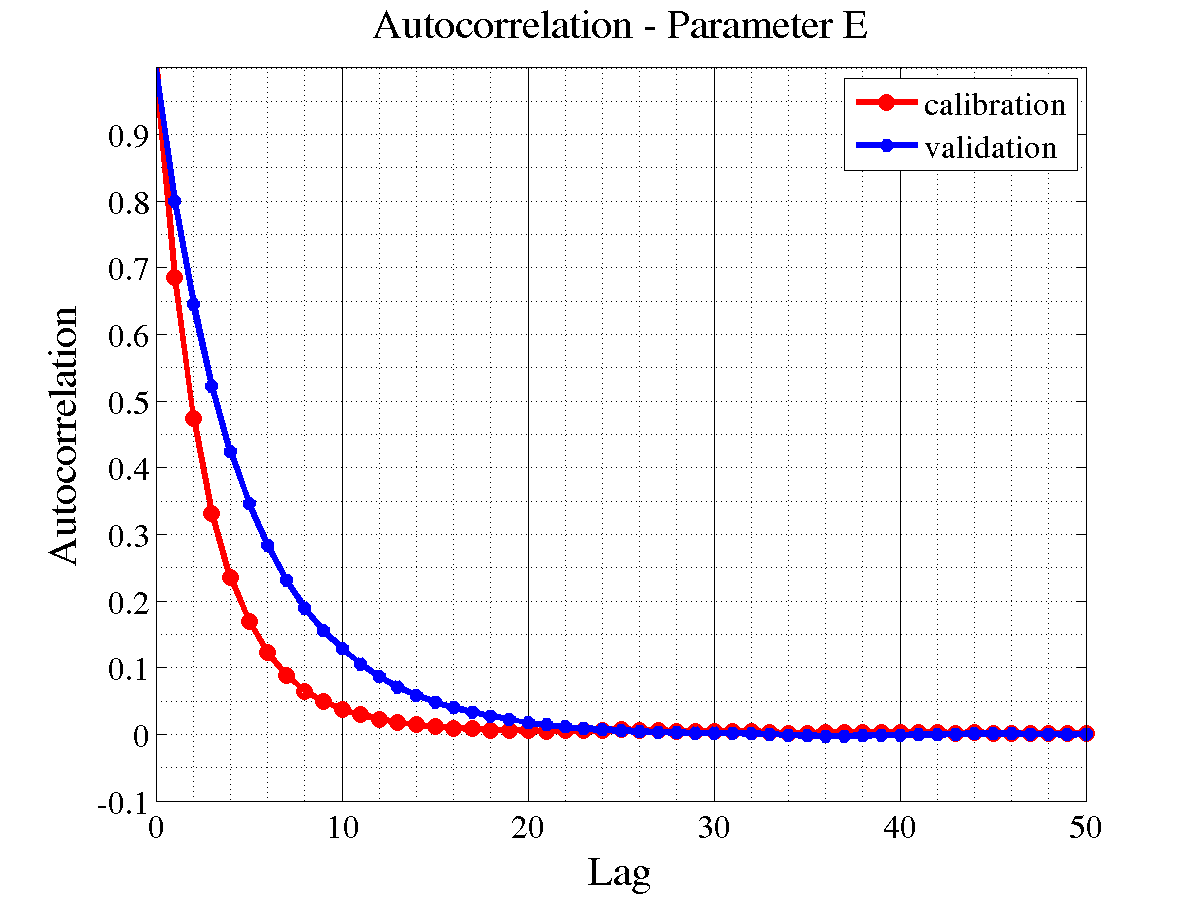
\includegraphics[scale=0.35]{figs/cal_val_parameter2_autocorrelation.png}}
\vspace*{-10pt}
\caption{Autocorrelation of parameters $A$ and $E$ (filtered chain).}
\label{fig:tga_ip_autocorrelation_param}
\end{figure}


\subsubsection{KDE, CDF and Autocorrelation Plots of QoI}
Figures \ref{fig:tga_pdf_qoi}  and \ref{fig:tga_cdf_qoi} present PDF and CDF of QoI, respectively and Figure \ref{fig:tga_autocorrelation_qoi} presents its autocorrelation.


\begin{figure}[htb]
\centering 
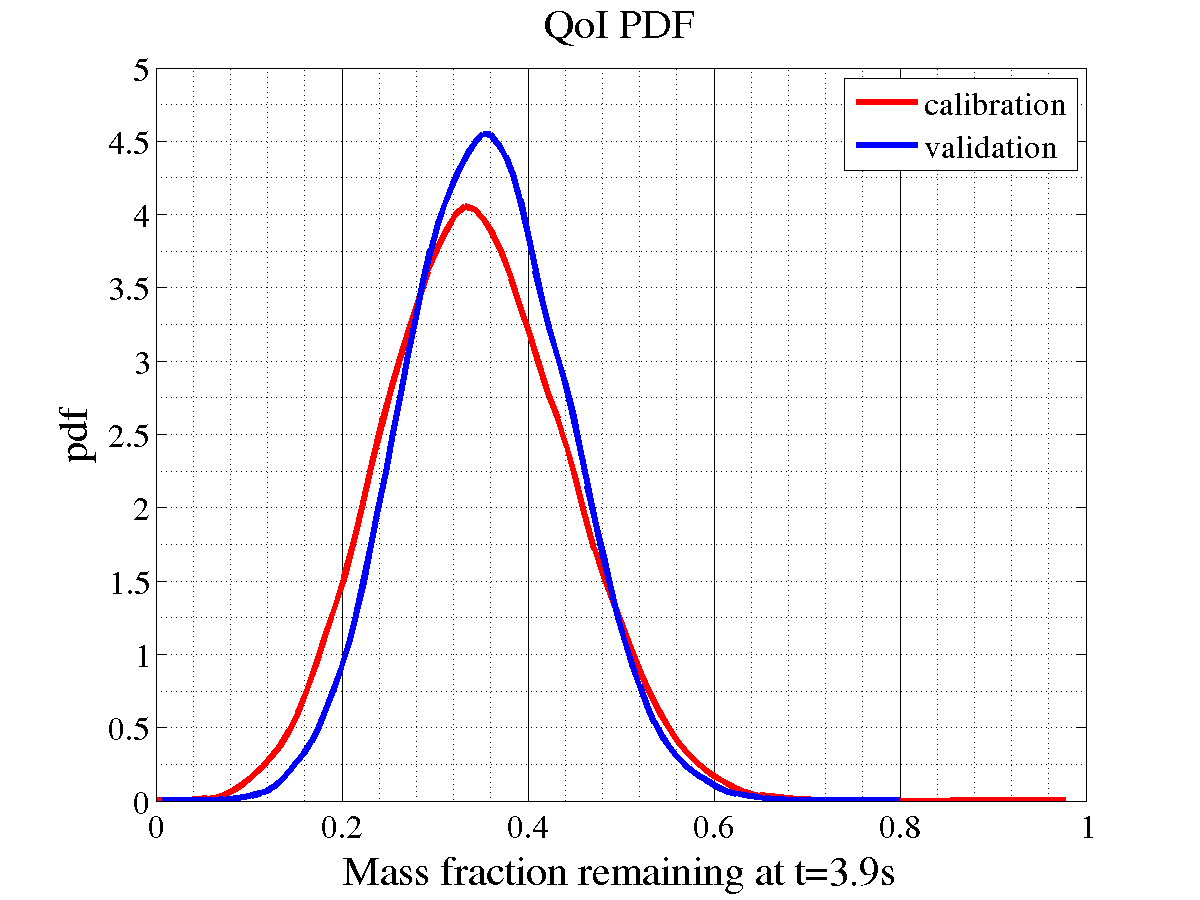
\includegraphics[scale=0.35]{figs/cal_val_QoI_PDF.png}
\vspace*{-10pt}
\caption{QoI PDF, during calibration and validation stages.}
\label{fig:tga_pdf_qoi}
\end{figure}



\begin{figure}[htb]
\centering 
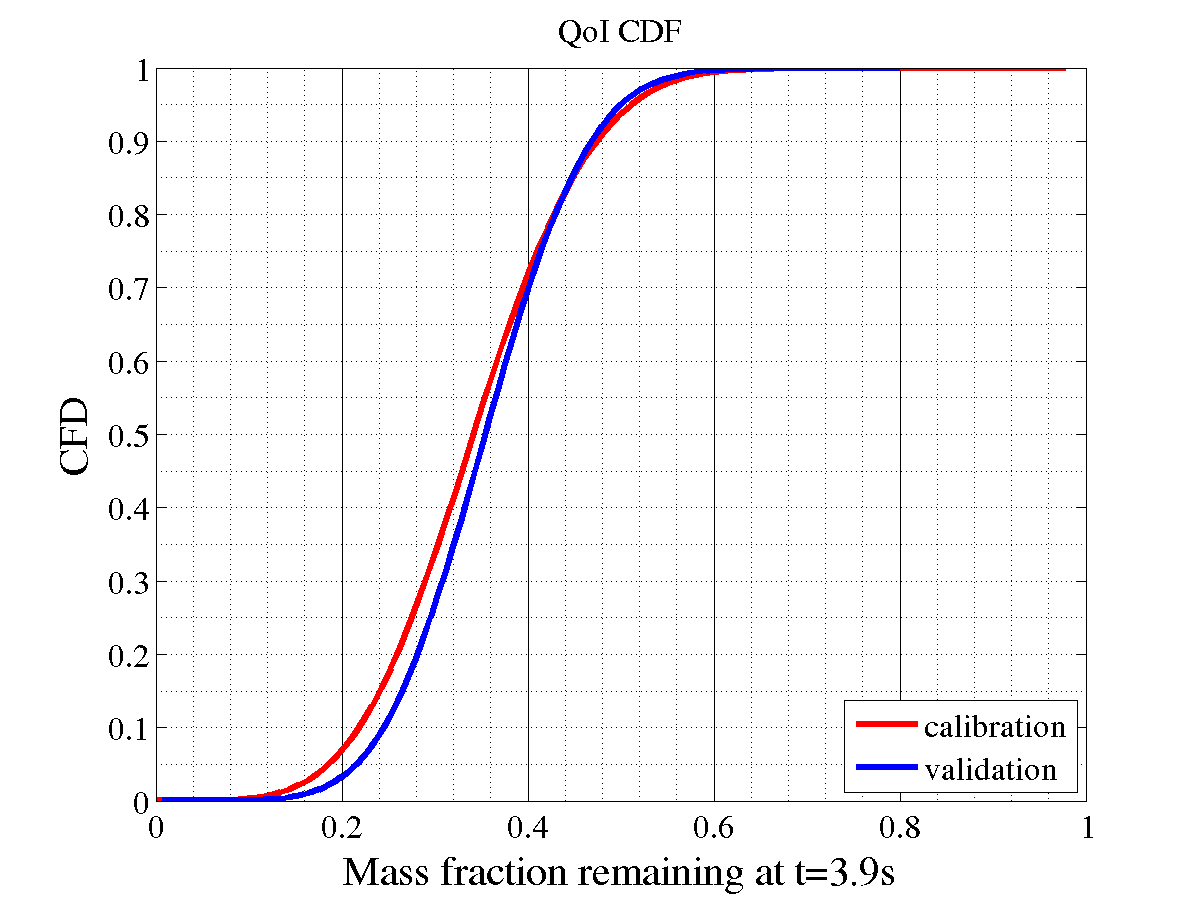
\includegraphics[scale=0.35]{figs/cal_val_QoI_CDF.png}
\vspace*{-10pt}
\caption{QoI CDF, during calibration and validation stages.}
\label{fig:tga_cdf_qoi}
\end{figure}

\begin{figure}[htb]
\centering 
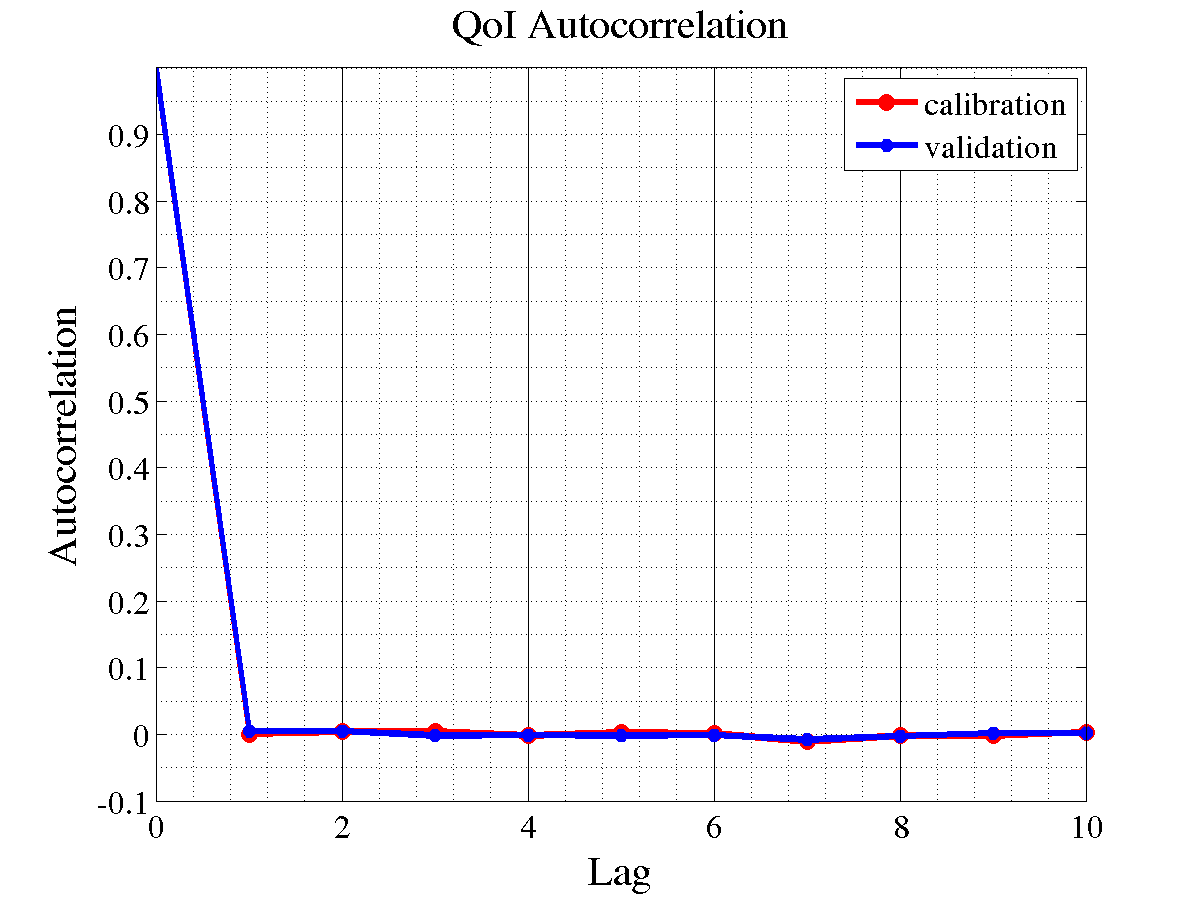
\includegraphics[scale=0.35]{figs/cal_val_QoI_autocorrelation}
\vspace*{-10pt}
\caption{QoI autocorrelation.}
\label{fig:tga_autocorrelation_qoi}
\end{figure}
